\begin{frame}{Algoritmos y técnicas utilizados}
	\begin{itemize}
		\item \textbf{Ingeniería de características. Selección y creación de características}
			\begin{itemize}
				\item Selección de variables semánticamente representativas. 
				\item LasVegas Wrapper. 
				\item Imputación de valores perdidos con media o mediana.
				\item Creación de características. \pause 
			\end{itemize}
		\item \textbf{Técnicas basadas en instancias. Selección, eliminación de ruido, sobremuestreo}
			\begin{itemize}
				\item ENN.
				\item IPF.
				\item SMOTE. Oversampling
				\item Random Undersampling. \pause 
			\end{itemize}
		\item \textbf{Ajuste de hiperparámetros.}
			\begin{itemize}
				\item Gridsearch de parámetros F (número de folds), N (mínimo peso de instancias) y O (número de ejecución para optimizar).
				\item 5-CV.
			\end{itemize}
	\end{itemize}
\end{frame}
\subsection{Técnicas que no dan resultados}
\begin{frame}{Malos resultados}
	\textbf{LasVegas Wrapper}
	\begin{itemize}
		\item Implementación en R (FSinR) que no consigue terminar una ejecución completa. \pause
	\end{itemize}
	\textbf{ENN, IPF}
	\begin{itemize}
		\item Limpieza de ruido empeora los resultados tanto en validación cruzada como test. Para ciertas configuraciones, incluso hacen desaparecer la clase minoritaria. 
	\end{itemize}
\end{frame}

\begin{frame}{Malos resultados}
	\textbf{SMOTE, Oversampling. Random Undersampling}
	\begin{itemize}
		\item Necesidad de 'numerizar' los datos. Creación de variables dummies. \pause
		\item Las técnicas de oversampling generan datos demasiado artificiales. En general, tienen accuracy cercano al 58\%.
	\end{itemize}
	\textbf{Imputación de valores perdidos o mal escritos} \pause
	\begin{itemize}
		\item \textit{Funder:} factor de 2141 niveles.
		\item \textit{Installer:} factor de 2411 niveles. 
		\item Muchos de esos niveles son resultado de escribir mal o de distintas formas la misma palabra.
		\item Reducción de los niveles hasta aproximadamente 500 corrigiendo los nombres, con peor precisión como resultado.
	\end{itemize}
\end{frame}

\subsection{Técnicas que dan resultados}

\begin{frame}{Buenos resultados}
	\textbf{Selección de características: Muchas columnas parecen inútiles}
	\begin{itemize}
		\item Elimino las variables \textit{wpt-name, subvillage, ward, recorded-by, scheme-name, num-private,region-code, quantity-group, source-type, waterpoint-type-group, payment-type} y \textit{extraction-type-group}
		\item Imputo valores perdidos en \textit{funder, installer, permit, scheme-management, public-meeting, gps-height, extraction-type.}
		\item Imputación de la variable \textit{construction-year} con los resultados de la validación cruzada en entrenamiento del mejor algoritmo hasta el momento (KNN).
	\end{itemize}
\end{frame}


\begin{frame}{Imagen del conjunto tras el preprocesamiento (TSNE)}
\begin{figure}
	\centering
	\includegraphics[scale=0.2]{figures/dat-ripper.png}
	\caption{Datos tras el preprocesamiento (TSNE)}
\end{figure}
	
\end{frame}

\begin{frame}{Mejor modelo}
	\begin{itemize}
		\item Ripper (JRip de RWeka) con variables \textit{latitude, longitude, date-recorded,basin,lga,funder,population,construction-year, gps-height,public-meeting,scheme-name,permit,extraction-type-class,management, management-group, payment, quality-group, quantity, source, source-type,source-class y waterpoint-type.}
		\item Hiperparámetros $F=2,N=3, O=29$.
	\end{itemize}
\end{frame}

\begin{frame}{Resultados}
\begin{itemize}
	\item 27 subidas. Mejor resultado: 0.7869.
	\item Mejor posición: 1752. Posición actual (17/02): 1834
\end{itemize}
	\begin{figure}
		\centering
		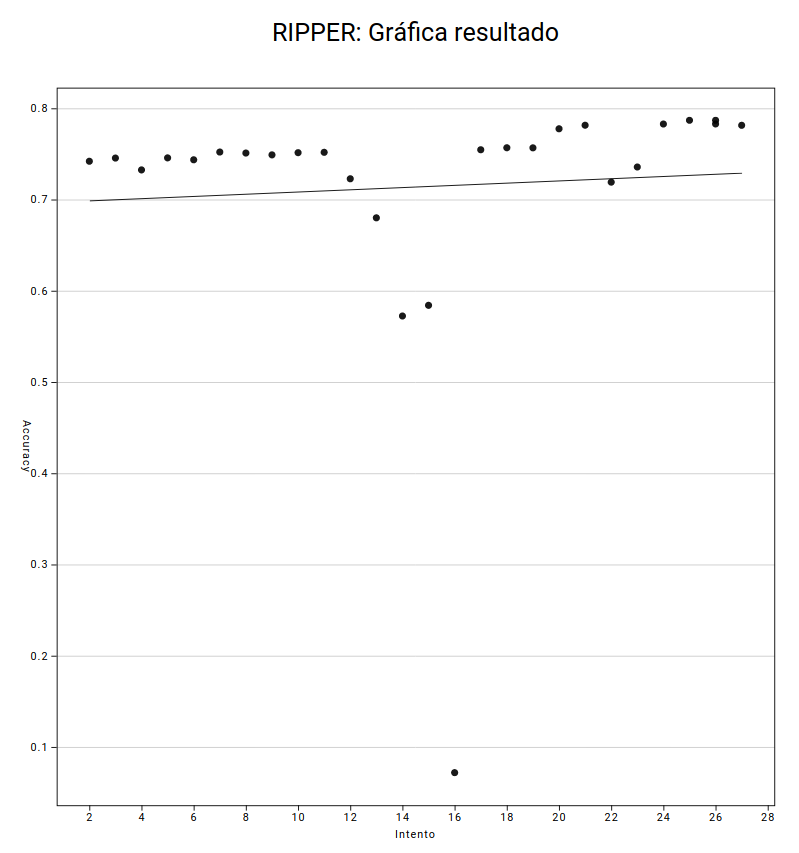
\includegraphics[scale=0.2]{figures/res-ripper.png}
		\caption{Gráfica de resultados}
	\end{figure}
\end{frame}

